\documentclass[a4paper,12pt]{article} 
\usepackage[french]{babel}
\usepackage[utf8]{inputenc}
\usepackage{answers}

\usepackage{hyperref}

\usepackage[table,xcdraw]{xcolor}
\usepackage{listings}
\definecolor{ForestGreen}{RGB}{34,139,34}

\usepackage{multicol}

\newcommand{\py}{\lstinline{Python} }

\definecolor{backcolour}{rgb}{0.95,0.95,0.92}

\lstset{%
	language         = Python,
	backgroundcolor  = \color{backcolour},
	basicstyle       = \ttfamily, % \upshape\ttfamily,
	keywordstyle     = \bfseries\color{blue}, %\bfseries,
	stringstyle      = \color{magenta},
	commentstyle     = \color{ForestGreen},
	alsoletter = > ,
	morekeywords = {>>>,as,assert,False,None, nonlocal,True, with,yield},
	showstringspaces = false,
	numbers=left,
	stepnumber=1,
	literate={à}{{\`{a}}}1 {é}{{\'e}}1 {è}{{\`{e}}}1 {ê}{{\^{e}}}1 {ç}{{\c{c}}}1 {Ç}{{\c{C}}}1,
}

\newcommand{\itemb}[1]{\item \textbf{#1}}

\usepackage{fancyhdr}  %package pour en-tetes et pied de pages
\usepackage{sectsty} % Permet de faire des modifications de police dans diverses sections des "headings" (cf. modif presentation de la page)
\pagestyle{fancy}       %Style pour en-tetes et pieds de pages
\fancyhead[CO,CE]{\sc Série 1\hspace{0.5mm}}
\fancyhead[RO,LE]{Collège Sismondi}  % LaTeX/TEX define \strut to be an invisible box of width zero that extends just enough above and below the baseline. Cela permet d'augementer légèrement la taille en bas de la box de manière à ce qu'elle soit collée à la ligne.
\fancyhead[LO,RE]{\small\ \textsl{1\textsuperscript{er} année - Informatique}}
\fancyfoot[RO,LE]{2021 - 2022}
\fancyfoot[LO,RE]{\small M.Schiess }
\fancyfoot[CO,CE]{\thepage}

\fancyhfoffset[l]{1.2cm} % le "l" en paramètre permet d'indiquer qu'on ne veut modifier que la marge à gauche.
\renewcommand{\headrule}{{%
		\hrule \headwidth \headrulewidth \vskip-\headrulewidth}}
\renewcommand\footrulewidth{\headrulewidth}
\renewcommand{\footrule}{{%
		\vskip-\footruleskip\vskip-\footrulewidth
		\hrule \headwidth \footrulewidth\vskip\footruleskip}}

\usepackage{tikz}
%-------------------------------------------------------------------------------
%---- Eclairage : en encadré sur fond jaune avec symbôle "ampoule" à gauche ----
%-------------------------------------------------------------------------------
\definecolor{coleclairage}{RGB}{255 , 221 , 156}
\definecolor{contoureclairage}{RGB}{255 , 192 , 0}
\newenvironment{eclairage}
{
	\begin{center}%
		\begin{tikzpicture}%
			\node[rectangle, draw=contoureclairage, top color=coleclairage!50, bottom color=coleclairage!140, rounded corners=5pt, inner xsep=5pt, inner ysep=6pt, outer ysep=10pt]\bgroup                     
			\begin{minipage}{0.98\linewidth}
				\begin{minipage}{0.08\linewidth}\centerline{
\includegraphics[scale=1]{../../theorie/Images/Symbole_eclairage.png}}\end{minipage}
				\begin{minipage}{0.89\linewidth}\itshape\footnotesize
				}
				{                		
				\end{minipage}
			\end{minipage}\egroup;%
		\end{tikzpicture}%
	\end{center}%
}

%-------------------------------------------------------------------------------
%---- apprendre : en encadré sur fond jaune avec symbôle "ampoule" à gauche ----
%-------------------------------------------------------------------------------
\definecolor{colapprendre}{RGB}{50,205,50}
\definecolor{contourapprendre}{RGB}{34,139,34}
\newenvironment{apprendre}
{
	\begin{center}%
		\begin{tikzpicture}%
			\node[rectangle, draw=contourapprendre, top color=colapprendre!10, bottom color=colapprendre!50, rounded corners=5pt, inner xsep=5pt, inner ysep=6pt, outer ysep=10pt]\bgroup                     
			\begin{minipage}{0.98\linewidth}
				\begin{minipage}{0.08\linewidth}\centerline{
\includegraphics[width=30px]{../../theorie/Images/Symbole_learn.png}}\end{minipage}
				\begin{minipage}{0.89\linewidth}\itshape\footnotesize
				}
				{                		
				\end{minipage}
			\end{minipage}\egroup;%
		\end{tikzpicture}%
	\end{center}%
}


%-----------------------------------------------------------------
%---- Modification présentation de la page: marges de la page ----
%-----------------------------------------------------------------
%\addtolength{\hoffset}{-1in}              % 1
%\addtolength{\voffset}{-1in}              % 2
\addtolength{\oddsidemargin}{-0.1 in} % 3
\addtolength{\evensidemargin}{-1in} % 3
\addtolength{\topmargin}{-1in}       % 4
\addtolength{\headheight}{6pt}       % 5
%\addtolength{\headsep}{-0.2cm}           % 6
\setlength{\textheight}{26cm}    % 7
\setlength{\textwidth}{16.5cm}      % 8
\addtolength{\marginparsep}{0pt}      % 9
\setlength{\marginparwidth}{0pt}   % 10
\addtolength{\footskip}{-1mm}           %11

\setlength{\parindent}{0em}% pas d'indentation


% Customiser le nom des sections
\usepackage{titlesec}
\titleformat{\section}[hang]{\Large \bfseries}{Série \thesection:\ }{0pt}{}

\renewcommand{\familydefault}{\sfdefault} % pour avoir des polices san serif

\newtheorem{Exc}{Exercice}
\Newassociation{correction}{Soln}{mycor}
\renewcommand{\Solnlabel}[1]{\bfseries Ex #1 }
\def\exo#1{%
	\futurelet\testchar\MaybeOptArgmyexoo}
\def\MaybeOptArgmyexoo{
	\ifx[\testchar \let\next\OptArgmyexoo
	\else \let\next\NoOptArgmyexoo \fi \next}
\def\OptArgmyexoo[#1]{%
	\begin{Exc}[#1]\normalfont}
	\def\NoOptArgmyexoo{%
		\begin{Exc}\normalfont}
		\newcommand{\finexo}{\end{Exc} \vspace{3mm}}
	\newcommand{\flag}[1]{}
	\newcommand{\entete}[1]

\newcommand{\getexocompteur}{{\the\numexpr \arabic{Exc}  \relax}}	
	
\newcommand{\eexo}{\vspace{5mm}} % espace pour séparer les exercices

\begin{document}
%		\title{\vspace{-3cm}Série 1}
%		\date{\vspace{-2cm}}
%		\maketitle

\fancyhead[CO,CE]{\sc Série \arabic{section} \hspace{0.5mm}}
\section{Représentation des nombres entiers}				
\Opensolutionfile{mycor}[cor_01]

\exo{}  ~\\ 
	\'Ecrire en base 10 les nombres suivants:
	\begin{multicols}{2}
		\begin{enumerate}
			\item $101_{(2)}$
			\item $10 000_{(2)}$
			\item $1111_{(2)}$
			\item $10101_{(2)}$
			\item $10_{(2)}$
			\item $111 000_{(2)}$
			
		\end{enumerate}
	\end{multicols}

	\begin{correction}
		~\\ \vspace{-7mm}
		\begin{multicols}{2}
			\begin{enumerate}
				\item $5$
				\item $16$
				\item $15$
				\item $21$
				\item $3$
				\item $56$
				
			\end{enumerate}
		\end{multicols}
	\end{correction}
\finexo

\exo{}  ~\\ 
	Les nombres suivants sont écrit en base 10. Donner leur écriture en base 2:
	\begin{multicols}{2}
		\begin{enumerate}
			\item 75
			\item 12
			\item 27
			\item 153
			\item 100
			\item 200
			\item 1000
			\item 2000
		\end{enumerate}
	\end{multicols}
	\begin{correction}
	~\\ \vspace{-7mm}
	\begin{multicols}{2}
		\begin{enumerate}
			\item $1001011_{(2)}$
			\item $1100_{(2)}$
			\item $11011_{(2)}$
			\item $10011001_{(2)}$
			\item $1100100_{(2)}$
			\item $11001000_{(2)}$
			\item $1111101000_{(2)}$
			\item $111110100011111010000_{(2)}$
		\end{enumerate}
	\end{multicols}
\end{correction}
\finexo

\exo{}  ~\\ 
	Écrire les nombres suivants en base hexadécimal:
	\begin{multicols}{2}
		\begin{enumerate}
			\item $10010010110_{(2)}$
			\item $111110_{(2)}$
			\item  $1000110101110101_{(2)}$
			\item $11110000000011_{(2)}$
		\end{enumerate}
	\end{multicols}
	\begin{correction}
	~\\ \vspace{-7mm}
	\begin{multicols}{2}
		\begin{enumerate}
			\item $496_{(16)}$
			\item $3E_{(16)}$
			\item  $8D75_{(16)}$
			\item $3C03_{(16)}$
		\end{enumerate}
	\end{multicols}
\end{correction}
\finexo

\exo{}  ~\\ 
	Écrire les nombres suivants en hexadécimal:
	\begin{multicols}{2}
		\begin{enumerate}
			\item 92
			\item 256
			\item  500
			\item 1023
		\end{enumerate}
	\end{multicols}
	\begin{correction}
	~\\ \vspace{-7mm}
	\begin{multicols}{2}
		\begin{enumerate}
			\item 60$_{(16)}$
			\item 100$_{(16)}$
			\item  1F4$_{(16)}$
			\item 3FF$_{(16)}$
		\end{enumerate}
	\end{multicols}
\end{correction}
\finexo

\exo{}[Compter en binaire]  ~\\ 
\begin{enumerate}
	\item Représenter en binaire les nombre 1, 2, 3, 4 et 5. Déduire une méthode pour compter en binaire.
	\item \textbf{En utilisant une seul main}, essayer de compter jusqu'à 31.
\end{enumerate}
\finexo

\exo{}  ~\\ 
\begin{enumerate}
	\item Combien de nombres peut-on représenter avec 8 bits? et 16 bits?
	\item Quel est le plus grand nombre qu'on peut représenter avec 8 bits? et 16 bits?
\end{enumerate}
	\begin{correction}
	~\\ \vspace{-7mm}
	\begin{multicols}{2}
		\begin{enumerate}
			\item C'est $2^{8}-1=255$ pour 8 bits et $2^16-1$=65535
			\item 100$_{(16)}$
		\end{enumerate}
	\end{multicols}
\end{correction}

\finexo


\exo{}[Envoyer des messages secrets]  ~\\ 
Tom est pris au piège à l’étage supérieur d’un grand magasin. Noël approche et il veut rentrer à la maison avec ses cadeaux. Que peut-il faire ? Il a essayé d’appeler, et même de crier, mais il n’y a plus personne. Il peut voir de l’autre côté de la rue quelqu’un qui travaille à l’ordinateur tard ce soir. Comment pourrait-il attirer son attention ? Tom regarde autour de lui et cherche ce qu’il pourrait utiliser. Il a alors une brillante idée : il peut utiliser les lumières de l’arbre de Noël pour lui envoyer un message ! Il trouve toutes les lumières et les branche de manière à pouvoir les allumer et les éteindre. Il utilise un code binaire simple, dont il est sûr que la personne de l’autre côté de la rue le comprendra.

Pouvez-vous le trouver ?
\begin{figure}[h]
	\begin{center}
		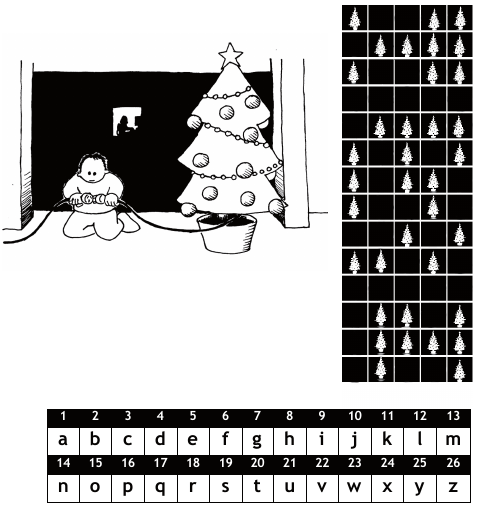
\includegraphics[scale=1]{images/send_secret_msg}
	\end{center}
\end{figure}

\finexo

% Solution		
		\newpage
		\setcounter{page}{1}
		\setcounter{section}{0}
		\Closesolutionfile{mycor}
		\titleformat{\section}[hang]{\Large \bfseries}{Corrigé Série \thesection:\ }{0pt}{}
		

		\fancyhead[CO,CE]{\sc Corrigé Série \arabic{section} \hspace{0.5mm}}
		\section{}
		\Readsolutionfile{mycor}
	\end{document}